\chapter{Appendix A}
\section{Hardware Virtualisation}
\label{ch:fundamentals/virtualisation/hardware-virtualisation}
\textcite{10.1145/361011.361073} refer to the control program as a \textit{virtual machine monitor} that 
ensures isolation and noninterference by providing every program with an environment that is \enquote{[...] effect
identical with that demonstrated if the program had been run on the original machine directly} 
\cite[2]{10.1145/361011.361073}. This definition implies that a running program does not directly use
the bare metal resources available. Instead, resources are emulated by the virtual machine monitor at
the hardware level and presented as a dedicated physical system. Such an environment is called 
a \textit{virtual machine}.

\begin{figure}[H]
    \centering
    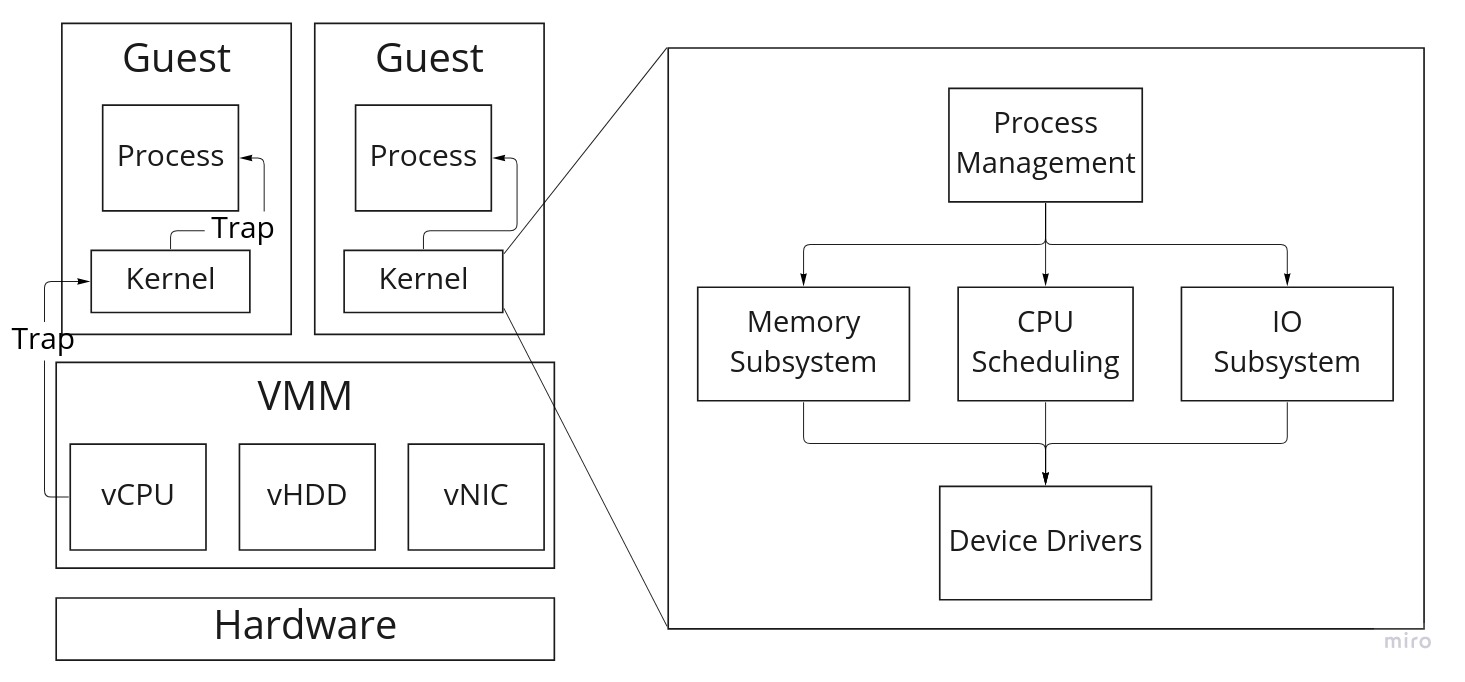
\includegraphics[width=0.70\textwidth]{images/fundamentals/full-virt-archh.jpg}
    \caption{Hardware virtualisation architecture. Each guest runs a complete operating system. 
             Privileged operations are trapped by the virtual machine monitor and emulated to provide hardware services.}
    \label{images:fundamentals/full-virt-archh.jpg}
\end{figure}

\textcite{10.1145/361011.361073} define a requirement that the instruction-set architecture of a computer
has to satisfy for it to be virtualisable. The instruction set must be segregated into three groups of
instructions - privileged, sensitive and innocuous. An instruction is privileged if it requires changing
the mode of execution from user to supervisor mode by means of a trap \cite{10.1145/361011.361073}. 
An instruction $i$ is control-sensitive if, when applied to the current processor state $S_1$, results
in a new state $i(S_{1}) = S_{2}$ such that the execution mode of $S_{2}$ does not equal that of $S_{1}$
or if $S_{2}$ has access to different resources than $S_1$ or both \cite{10.1145/361011.361073}. 
An instruction is behaviour-sensitive if its execution depends on the execution mode or its position
in memory \cite{10.1145/361011.361073}. An instruction is innocuous if it is not sensitive. 
Given these definitions, a computer is virtualisable \enquote{[...] if the set of sensitive instructions
for that computer is a subset of the set of privileged instructions} \cite[6]{10.1145/361011.361073}.
If this criterion is met, the virtual machine monitor can trap all sensitive instructions and emulate 
each via a homomorphism $i: C_{r} \rightarrow C_{v}$ that maps the state space of the processor without
the virtual machine monitor loaded $C_{r}$ to the state space with the virtual machine monitor loaded 
$C_{v}$ \cite{10.1145/361011.361073}. Innocuous instructions do not require protection, i.e a homomorphic
mapping, and are directly executed by the processor \cite{10.1145/361011.361073}.

Given the aforementioned homomorphism, a virtual machine can host a \textit{guest kernel} (Figure \ref{images:fundamentals/full-virt-archh.jpg}) that 
runs completely in user mode. 
Whenever the guest kernel attempts to execute a privileged instruction, 
the virtual machine monitor traps the attempt and emulates the instruction. 
Consequently, the guest kernel does not have to be a part of the trusted computing base. 
Even if it is compromised or encounters an unrecoverable error condition, other virtual machines 
remain unaffected. As a result, the isolation boundary between user programs running in different 
virtual machines is stronger compared to processes running on a shared kernel. 

In order to fully guarantee spatial noninterference between processes, the virtual machine monitor must 
be in full control of the host system's memory. There are two primary methods to do this - 
\textit{shadow paging} and \textit{extended page tables}. The former mechanism is considered first. 
The virtual machine monitor maintains a nested page table 
per guest, also called a \textit{shadow page table} \cite{10.5555/1204009}. 
In turn, the guest kernel maintains a page table per process. 
Whenever the guest kernel schedules a new process for execution, it modifies the \textit{page-table 
base register} to point to the page table for that process \cite{10.5555/1204009}. 
The virtual machine monitor intercepts this attempt and transparently updates the page table pointer to point to 
the guest's shadow page table corresponding to that process \cite{10.5555/1204009}. Note that 
the virtual machine monitor has to traverse the shadow page table for that guest in order to find the nested entry corresponding 
to the process. Afterwards, the memory management unit takes care of translating the virtual memory 
addresses of the guest and updating the \textit{translation lookaside buffer}.
Alternatively, the memory management unit may be \enquote{virtualisation-aware} in the sense that it knows 
there are two page tables it needs to traverse - the page table that maps guest virtual memory to guest 
\enquote{physical memory}, and the page table that maps guest physical memory to actual physical memory. 
The former is maintained by the guest kernel, whilst the latter is maintained by the virtual machine monitor.
The extended page table approach is up to 50\% faster than shadow paging \cite{2006PerformanceEO} because table
walks are done in hardware - by the memory management unit.
Nevertheless, maintaining page table data structures inside the virtual machine 
monitor and the guests leads to memory pressure, which is further amplified by the fact that 
guests, their applications and the virtual machine monitor all share the same physical memory \cite{10.5555/2490781}. 

The spatial noninterference property necessitates that the virtual machine monitor manage 
all input-output devices and their interactions with the guests. This is accomplished by the
already introduced trap-and-emulate pattern. When an application within a virtual machine 
issues a system call requesting some form of input-output, the request is processed by the 
I/O stack inside the guest. At the lowest level of the stack, the device driver issues a 
command to the device, typically by writing to memory specifically assigned to the device, or by
calling specific input-output instructions \cite{10.5555/2490781}. 
Either way, the virtual machine monitor intercepts this and traverses its own I/O stack, which 
remaps guest and real input-output addresses and forwards the request to a physical device \cite{10.1145/2063176.2063194}. 
After processing the request, the physical device triggers an interrupt that is caught by the virtual machine monitor and 
transformed into a virtual equivalent that is sent to the virtual machine that issued the request.
To reduce the overhead associated with interrupt processing, the virtual machine monitor can batch 
multiple events together and use a single interrupt to notify the guest kernel \cite{10.1145/2063176.2063194}.
Still, a request must traverse two input-output stacks. The same holds for the response.
In addition, hardware optimisations such as direct memory access are emulated in software, which 
further degrades performance. This, however, can be mitigated by integrating an input-output memory management 
unit that remaps all direct memory accesses of a device on the host to an address space in the guest.

The cost of hardware virtualisation becomes apparent when measuring same-host density
and boot times. \textcite{10.1145/3132747.3132763} consider memory consumption and on-disk image size
as the primary limiting factors. The authors measure the time it takes to create and boot
virtual machines using the Xen virtual machine monitor and show the negative effects that on-disk image size has 
by starting images with 
varying sizes by manually \enquote{[...] injecting binary objects into the uncompressed image file} \cite[3]{10.1145/3132747.3132763}. 
As the number of consolidated virtual instances increases and the image size grows, 
creation and boot times increase linearly.
Furthermore, the authors show that creating and starting a process directly on the host is, on average, 
two orders of magnitude faster. \textcite{10.1145/2151024.2151030} also evaluate Xen and state
that processing units spend 25\% of their total cycles in hypervisor mode instead of executing guest applications 
when running \enquote{[...] SPEC's first benchmark addressing performance evaluation of datacenter servers used in 
virtualised server consolidation} \cite[2]{10.1145/2151024.2151030}, which includes components 
such as a web, database and application server.

\section{Container configuration}

\begin{lstlisting}[style={syscalls}, label={code:oci-config.json}, caption={Open Containers Initiative Configuration File Example}]
{
    "process": {
        "args": [
        "nsbench-disk-workload"
        ],
        "cwd": "/"
    },
    "root": {
        "path": "./workloads/rootfs/disk",
        "readonly": false
    },
    "namespaces": [
        {
        "type": "user"
        },
        {
        "type": "net"
        },
        {
        "type": "ipc"
        },
        {
        "type": "mnt"
        },
        {
        "type": "uts"
        },
        {
        "type": "pid"
        }
    ],
    "uid_mappings": [
        {
        "container_id": 0,
        "host_id": 1000,
        "size": 1
        }
    ],
    "gid_mappings": [
        {
        "container_id": 0,
        "host_id": 1000,
        "size": 1
        }
    ],
    "hostname": "nsbench-disk-workload",
    "hooks": { 
        "on_runtime_create": [
            {
                "path": "/usr/bin/setup-network",
                "args": ["-a", "192.168.0.101"],
                "env": ["PATH=/usr/bin"],
                "timeout": 2
            }
        ],
        "on_container_created": [],
        "on_container_start": [],
        "on_container_started": [],
        "on_container_stopped": []
    }
}
\end{lstlisting}

\begin{lstlisting}[style=c-code-snippets, label={code:implementation/benchmark/network-hook-doer}, caption={Joining an arbitrary namespace, executing a function within it, and returing back to the original namespace}]
func DoInContainerNamespace(containerPid, namespace int, doer func() error) error {
    runtime.LockOSThread()
    defer runtime.UnlockOSThread()

    ns, ok := namespaces[namespace]
    if !ok {
        return ErrNamespaceUnsupported
    }

    oldNsPath := path.Join("/proc", "self", "ns", ns)
    oldNsFd, err := unix.Open(oldNsPath, unix.O_RDONLY|unix.O_CLOEXEC, 0)
    if err != nil {
        return err
    }
    defer unix.Close(oldNsFd)

    newNsPath := path.Join("/proc", strconv.Itoa(containerPid), "ns", ns)
    newNsFd, err := unix.Open(newNsPath, unix.O_RDONLY|unix.O_CLOEXEC, 0)
    if err != nil {
        return err
    }
    defer unix.Close(newNsFd)
    if err := unix.Setns(newNsFd, namespace); err != nil {
        return err
    }
    defer unix.Setns(oldNsFd, namespace)
    return doer()
}
\end{lstlisting}

\section{Netlink protocol}
\label{ch:appendix/netlink-protocol}

\clearpage